\documentclass[a4paper]{article}

%% Language and font encodings
\usepackage[english]{babel}
\usepackage[utf8x]{inputenc}
\usepackage[T1]{fontenc}

%% Sets page size and margins
\usepackage[a4paper,top=3cm,bottom=2cm,left=3cm,right=3cm,marginparwidth=1.75cm]{geometry}

%% Useful packages
\usepackage{amsmath}
\usepackage{graphicx}
\usepackage{wrapfig}
\usepackage[colorinlistoftodos]{todonotes}
\usepackage[colorlinks=true, allcolors=blue]{hyperref}

\title{Best Laid Plans of Lions and Men}
\author{Danny Rademacher, Jens Harder}

\begin{document}
\maketitle

%%%%%%%%%%%%%%%%%%%%%%%%%%%%%%%%%%%%%%%%%%%%%%%%%%%%%%%%%%%%%%%
%%                                                           %%
%%                                                           %%
%%  https://www.overleaf.com/10975949ttqhccgxsxmn#/41322390/ %%
%%                                                           %%
%%                                                           %%
%%%%%%%%%%%%%%%%%%%%%%%%%%%%%%%%%%%%%%%%%%%%%%%%%%%%%%%%%%%%%%%

\newpage
\tableofcontents
\newpage
\section{Introduction}

During the lab `Computational Geometry` (SS 2017)in the university of Bonn we designed an applet to visualize
the algorithm in `Best Laid Plans of Lions and Men` \cite{paper}. This paper describes two different configurations for the Man and Lions Problem, the first in a bounded area, represented with a graph, and the second one in the plane.\\
Our intention was to visualize both configuration and the described algorithms, to easily explain their routines. Furthermore we extended the problem on the graph with more algorithms and parameter, to explore more characteristics of the problem.\\
\\
In this documentation will give a short overview over the problems itself and will explain how to use the applet.


\section{Lions and Men Problem}

In the Lions and Men Problem, $n$ lions try to catch $m$ men in a special invironment. The men try to escape as long as possible, against all possible lion strategies. \cite{paper} gives for two different environments (special graph and plane) man strategies to escape always all lions.

\subsection{On a graph}

The first configuration describes a special designed graph, so that one man can always escape two lions, independent of the lion strategies. The man runs from $quarter$ to $quarter$  and decides with only the current lion positions, where to go next (without knowing the future steps of the lions).\\
In this special graph (see figure \ref{fig:specialGraph}) each vertex has 3 incident edges and each edge has weight 4. This means that an entity (man or lion) needs 4 steps to run from one vertex to one of the neighbor vertices. A $quarter$ of an edge is an edge step which is next to a vertex. 

\begin{figure}[hbt]
  \centering
    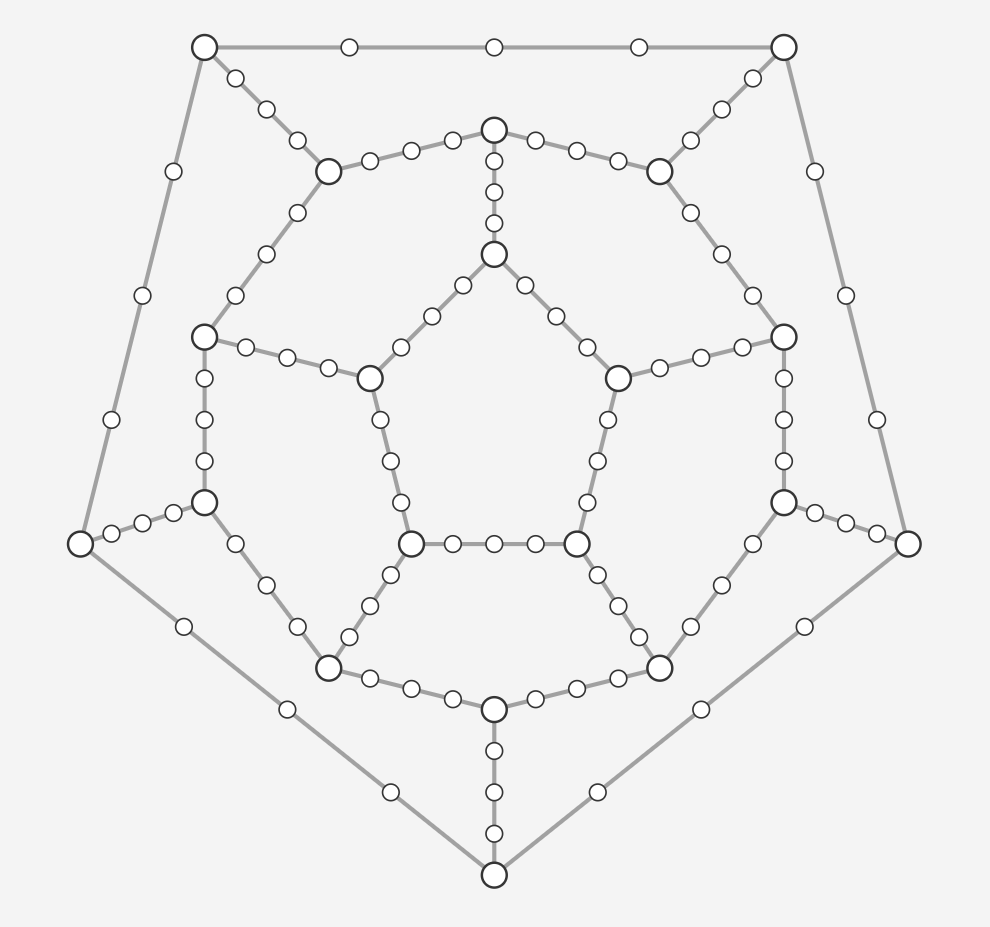
\includegraphics[width=0.55\textwidth]{specialGraph.PNG}
  \caption{Special designed graph in \cite{paper}}
  \label{fig:specialGraph}
\end{figure}

\subsection{In the plane}
This configuration is in the $R^2$ plane. All n lions move around the plane with $speed = 1$ to catch one man. The man has $speed \epsilon > 1$.
\cite{paper} provides an algorithms, in which the man can always escape the lions, if the startingposition of all lions is different to the starting position of the man. Note: If the man escapes the convex hull of all lions, he succeeded, because is has higher speed then the lions.\\
The idea of the algorithm is, that to make an induction about all lions. In the first step the algorithm is trivial. The man runs in the opposite direction of the lion and escapes. From now on the man tries to run the same path as in the previous induction step if possible. If there is a lion onhis way, the man makes a special move to avoid the lion. If the move has sourounded the lion, the man continues on the original path, until there is another lion to surround, or the man escaped all lions successfullly. It is important, that the man gets more speed each induction step (to maximal $1 + \epsilon speed$), so that all lions in the earlier induction steps can be ignored.


\section{The Applet}
When starting the applet, you get to the main screen where you can choose which part of the applet to use. There are to different parts: the "Lions On Graph" part (section \ref{sec:applet_graph}) and the problem "Lions In Plane" (section \ref{sec:applet_plane}. You can switch between both parts any time, using the "Choose App" button in the bottom right corner.

\subsection{Lions On Graph}\label{sec:applet_graph}

\subsubsection*{Create and modify the graph}

\begin{wrapfigure}{r}{0.36\textwidth}
  \vspace{-20pt}
  \begin{center}
    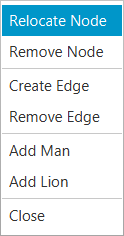
\includegraphics[width=0.25\textwidth]{modify.png}
  \end{center}
  \vspace{-20pt}
  \caption{Modify a graph}
  \label{fig:modify}
  \vspace{-10pt}
\end{wrapfigure}
If you choose "Lions In Plane", you see an empty screen. With "Set Graph" you can open an existing graph, load a graph file (if available) to create your own graph. \\
To create or modify a graph, you need to right click on the corresponding place. For example to create a new vertex: do a right click on an empty place and choose "Add Node". To create an new edge click on an existing node (see figure \ref{fig:modify}), choose "Create Edge" and do a left click on the target node. To modify (change edge weight, relocate vertex, ...) do a right click on the corresponding shape.\\

\subsubsection*{Create and modify the entities}
To create, remove or relocate entities (lions and men), do a right click on a vertex or on the entity itself. Furthermore you can change the entity properties such as the strategy or the range. Just click on the property and select the new value / insert it in the popup).

\subsubsection*{Usage}
After you created the graph with the entities (see figure \ref{fig:graphConfig}, you can go to the "Play Mode" (bottom left corner).
\begin{figure}[hbt]
  \centering
    
\includegraphics[width=0.8\textwidth]{play.PNG}
  \caption{Different play options}
  \label{fig:play}
\end{figure}
In the "Play Modus", you can start the complete animation ("Play"), do the animation step by step ("Single Step") or change the animation speed. You can also change which parts of the entities should be visible. See figure \ref{fig:play}.\\
If one of the strategies is "Manual" you can choose each step where to move this entity. Note: During the "Play Mode" it is not possible to change entity properties (such as the strategy) or to modify the graph. To change the setup you need to go back to the "Edit Mode" (bottom left corner)

\begin{figure}[hbt]
  \centering
    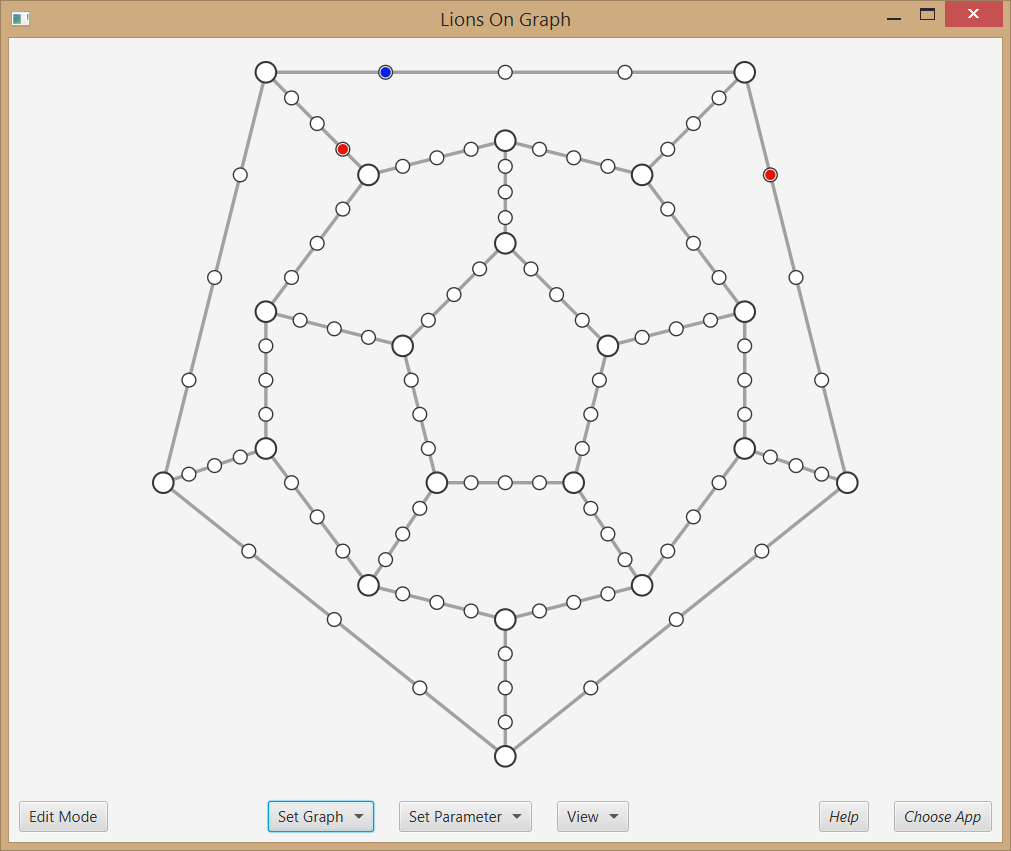
\includegraphics[width=0.8\textwidth]{graphApplet.PNG}
  \caption{Example Configuration. The special graph from \cite{paper} with one man (blue) and two lions (red).}
  \label{fig:graphConfig}
\end{figure}

\subsection{Lions In Plane}\label{sec:applet_plane}

\subsubsection*{Create and modify the plane}
Analogous to the "Lions On Graph" applet, you can modify the plane with right click. Right click on a empty place you can add a new lion or the man. With a right click on an entity you can relocate the entity or change the strategy. If you added multiple lions, you can see the green polygon which is the convex hull of all lions. To escape all lions, the man needs to escape from the convex hull. This is enough, because the man is $\epsilon > 0$ faster then the lions.

\subsubsection*{Usage}
If you created all lions and the man (see figure \ref{fig:planeConfig}, you can go to the "Play Mode" (bottom left corner). 
\begin{figure}[hbt]
  \centering
    
\includegraphics[width=0.8\textwidth]{play.PNG}
  \caption{Different play options}
  \label{fig:play}
\end{figure}
In the "Play Modus", you can start the complete animation ("Play"), do the animation step by step ("Single Step") or change the animation speed. You can also change which parts of the entities should be visible. See figure \ref{fig:play}.\\
\begin{figure}[hbt]
  \centering
    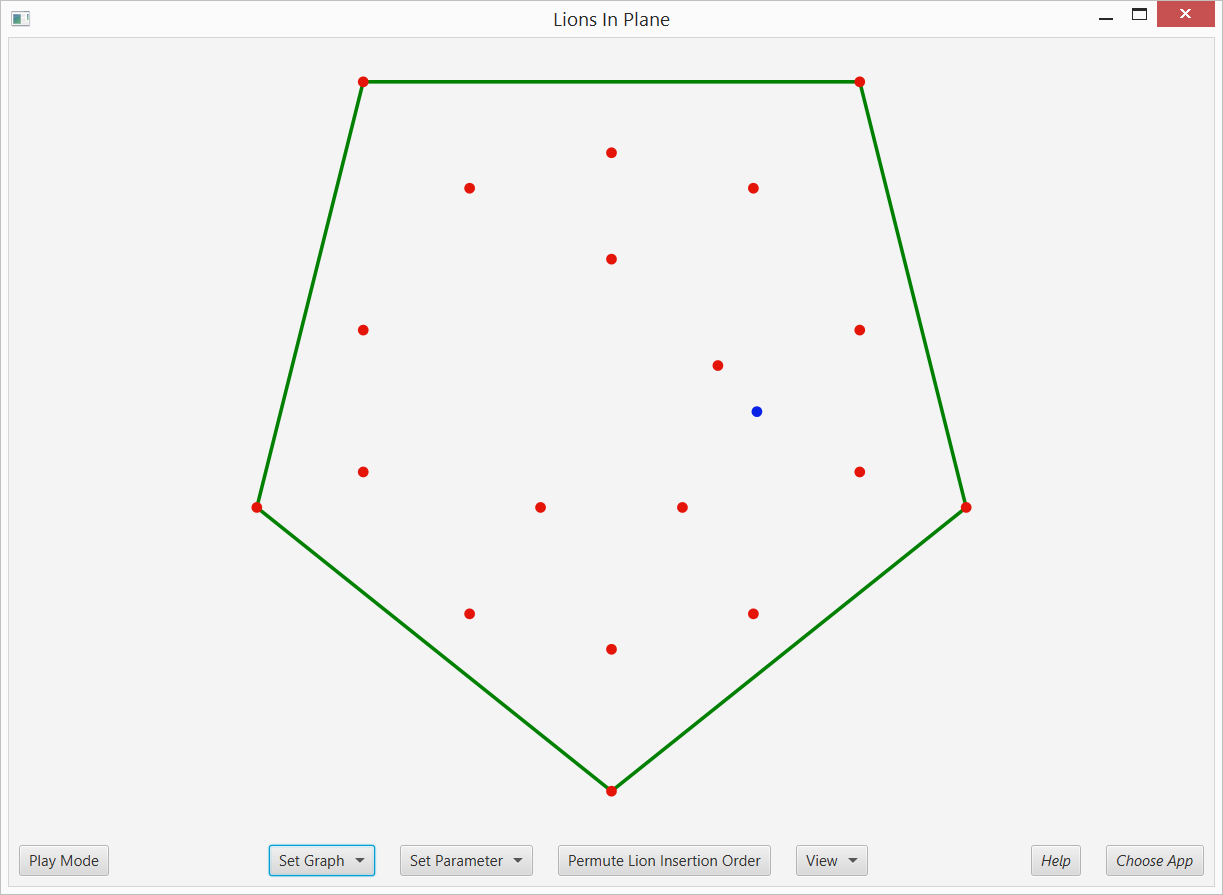
\includegraphics[width=0.8\textwidth]{planeApplet.PNG}
  \caption{Example Configuration. The plane with one man (blue) and multiple lions (red). You can see the convex hull of the lions (green)}
  \label{fig:planeConfig}
\end{figure}
\begin{figure}[hbt]
  \centering
    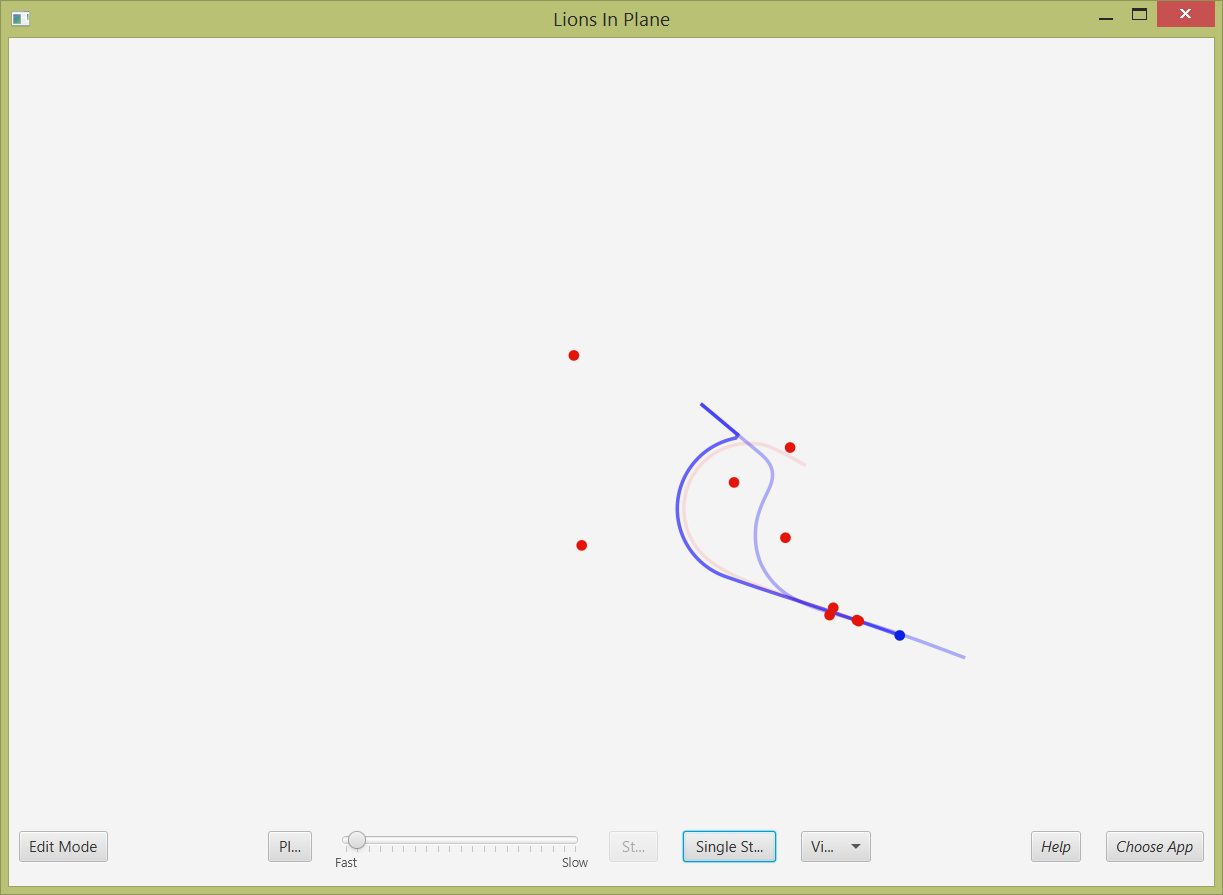
\includegraphics[width=0.8\textwidth]{planeAppletRun.PNG}
  \caption{During the animation. You can see the man path from the last induction step (light blue), the man path from the current induction step (blue) and the lion path from the current lion (light red). All lions are red points and the man is the blue point.}
  \label{fig:planeConfigPlay}
\end{figure}
With "View" you can decide which shapes / paths should be visible in the applet. During the animation, the applet shows the current induction step and goes to the next induction step, until the induction over all lions is completed (see figure \ref{fig:planeConfigPlay}). Note: Is is not possible to add, remove or change entities in the "Play Mode". You have to go back to the "Edit Mode" to modify the setup.



\newpage
%	\defaultsectionstyle	
	\begin{thebibliography}{99}
		
		
		\bibitem[Ab17]{paper} \textsc{M. Abrahamsen, J. Holm, E. Rotenberg, C. Wulff-Nilsen} (2017): Best Laid Plans of Lions and Men. (SOCG'17) arXiv:1703.03687 [cs.CG]

	

		
	\end{thebibliography} 



\end{document}